% ========== SIGNAL AND CONROL REGIONS DEFINITION SECTION ==========

% Intro and motivation
Given the analysis region selection from Section \ref{sec:vzy-selection} and the
\ac{BDT} discriminant developed in Section \ref{sec:vzy-bdt}, additional
selection cuts can be added to define signal and control regions for use in
the fit. By applying tighter selections in constructing the
\ac{SR}, the analysis' sensitivity to the signal process is improved.
Additionally, the use of orthogonal \acp{CR}
with minimal signal leakage enables data-\ac{MC} comparisons before
unblinding, to confirm validity of background modelling, and also gives the fit
more data with which to constrain systematic uncertainties.

% Variables used
\newcommand\rarsig{\ensuremath{\mathcal{R}^\text{sig}_\text{BDT}}\xspace}
One \ac{SR} and three \acp{CR} are used for this analysis. The four regions are
divided by two variables: $m_{jj}$ and signal rarity. Signal rarity, or
\rarsig, is a transformation of the \ac{BDT} output defined in Section
\ref{sec:methods-bdt-output}.
These two variables are plotted in Figure \ref{fig:vzy-srcr-cutdists}, for
events in the analysis region.

\begin{figure}[tb]
  \centering
  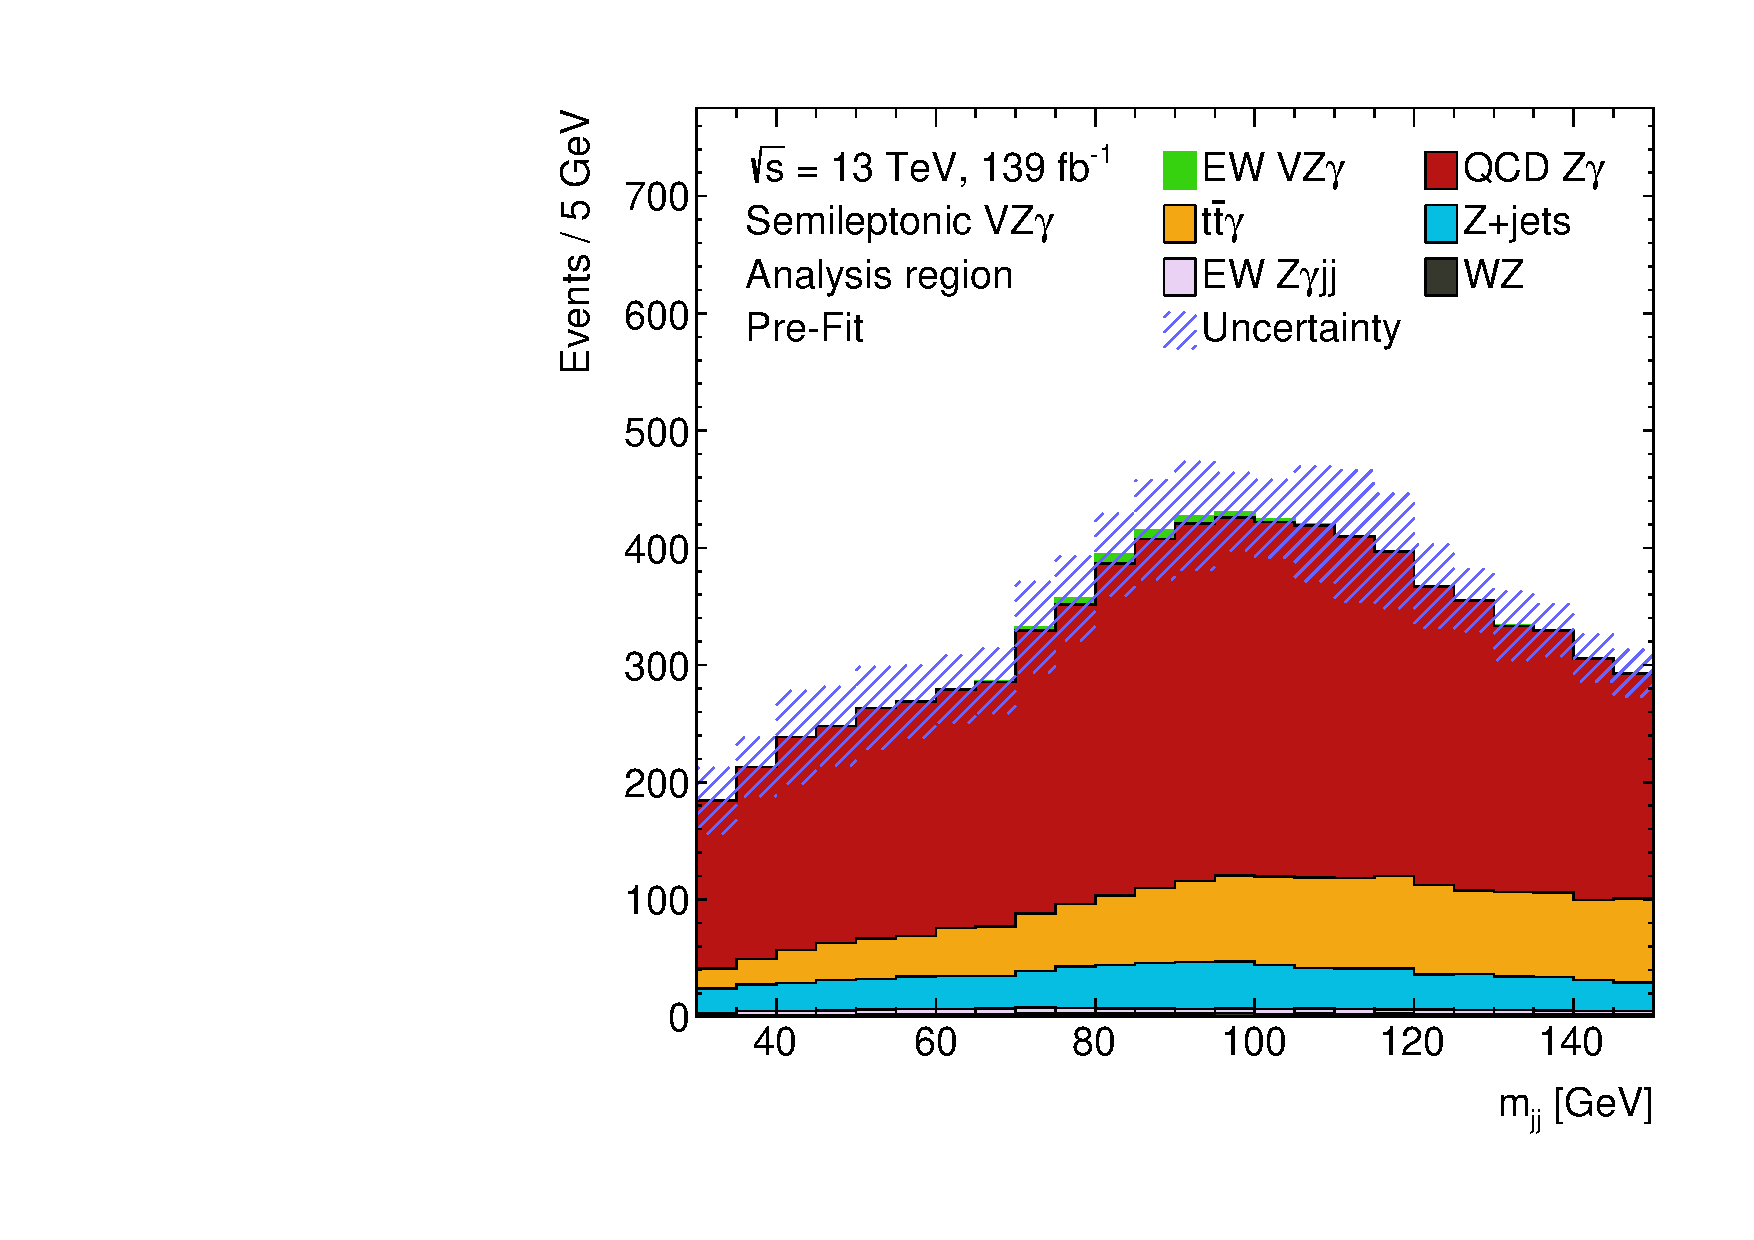
\includegraphics[width=.495\textwidth]{\resource{stack/AR_mjj.pdf}}
  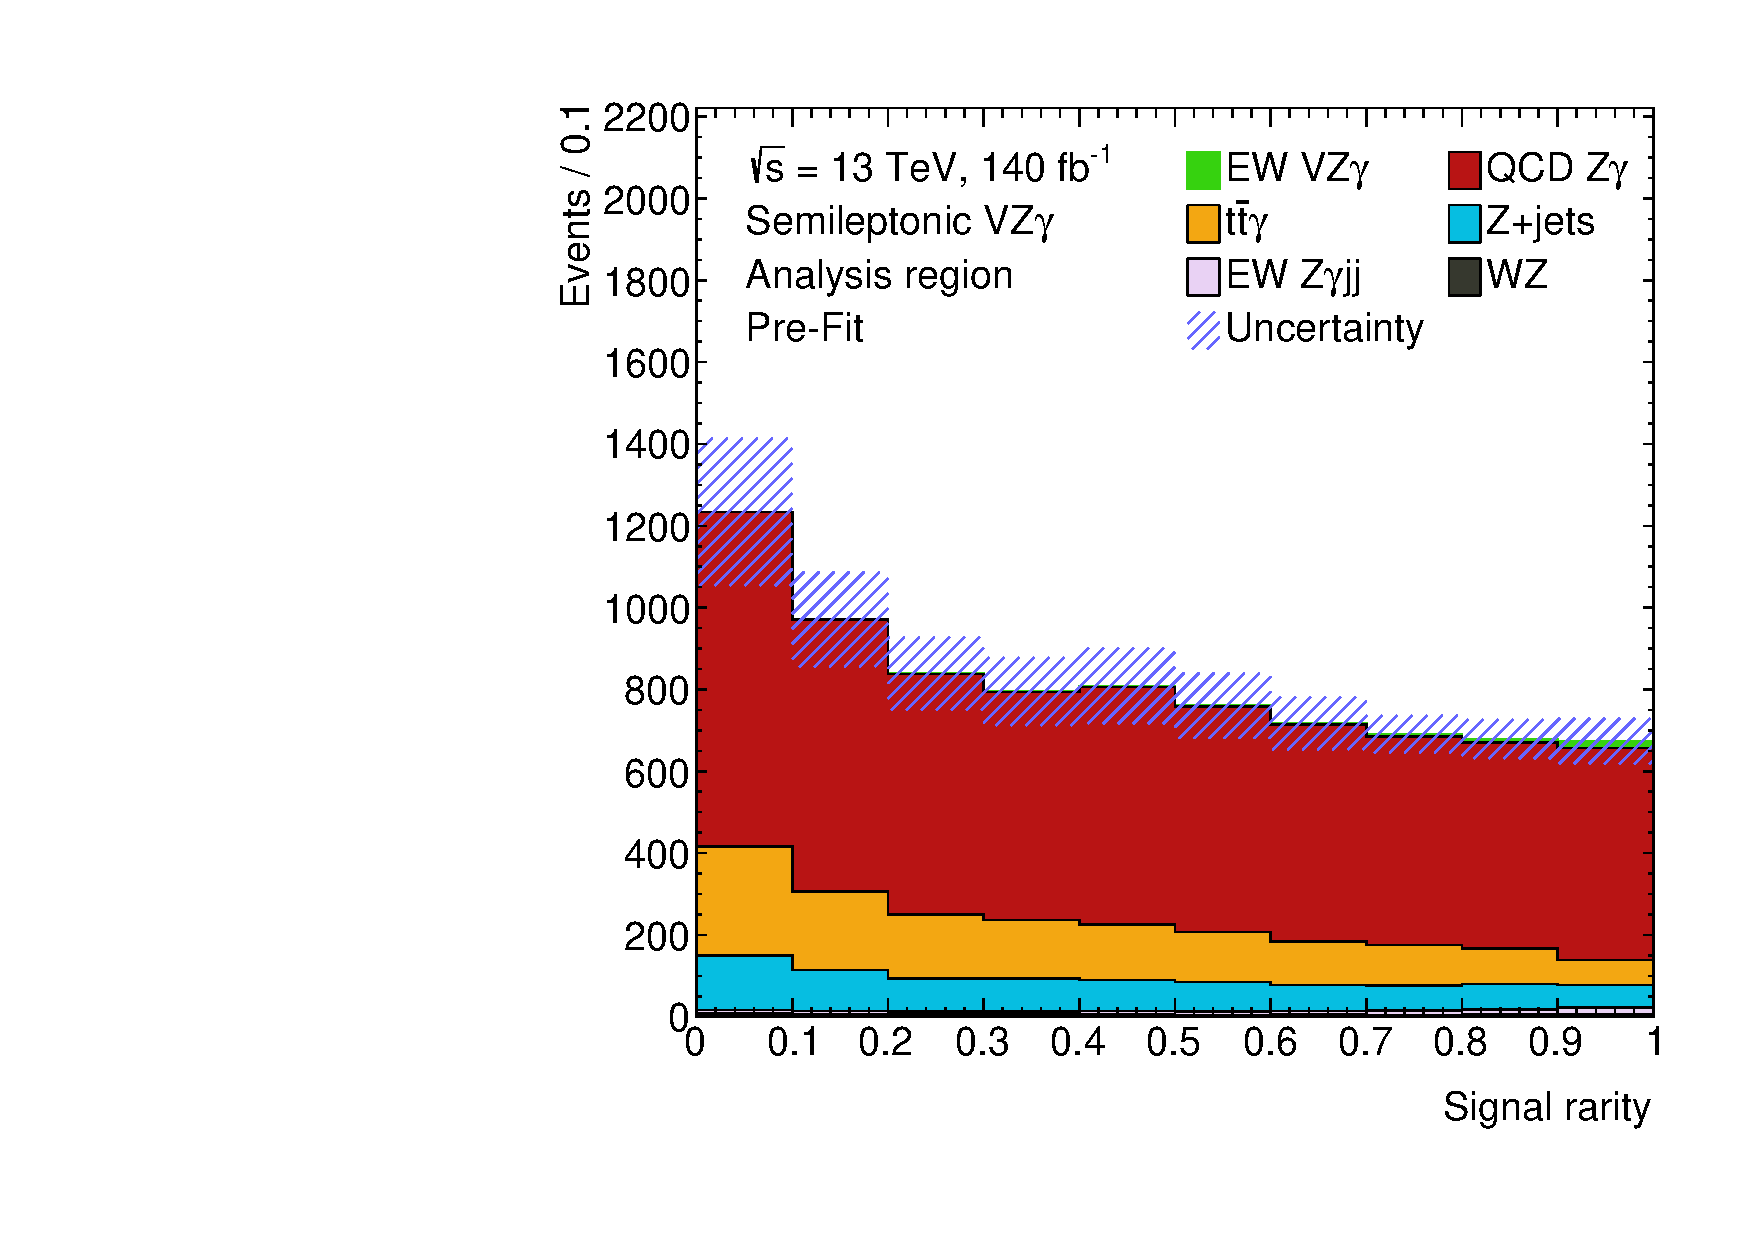
\includegraphics[width=.495\textwidth]{\resource{stack/AR_BDT.pdf}}
  \caption{
    Distribution of dijet mass (left) and signal rarity (right) for events
    in the analysis region, defined by the selection in Table
    \ref{tab:vzy-selection}. Yields for the signal process and all backgrounds
    are shown stacked. The error band represents the total
    pre-fit uncertainty from all sources of systematic uncertainty.
  }
  \label{fig:vzy-srcr-cutdists}
\end{figure}

\begin{figure}[tbh]
  \centering
  \includegraphics[width=.9\textwidth]{\resource{m_jj_window_scan.pdf}}
  \caption{
    Approximate significance calculated with $s/\sqrt{b}$ for a number of signal
    events $s$ and background events $b$ with an $m_{jj}$ value between the
    minimum value given on the $x$-axis and the maximum on the $y$-axis.  The
    number of signal events is calculated from the \acs{EW} \VZy sample and all
    background samples are included for the background estimate.  Events are
    required to pass the analysis region selection from Table
    \ref{tab:vzy-selection}. The maximum significance is obtained for a cut of
    $70 < m_{jj} < 100$ GeV.
  }
  \label{fig:vzy-srcr-mjjscan}
\end{figure}

\begin{figure}[tbh]
  \centering
  \includegraphics[width=.9\textwidth]{\resource{m_jj_cut_schematic.pdf}}
  \caption{
    Illustration of the three $m_{jj}$ regions used in the analysis: the lower
    sideband ($30 < m_{jj} < 65$ GeV), the upper sideband ($110 < m_{jj} < 150$
    GeV), and the peak ($70 < m_{jj} < 100$ GeV) region which is then subdivided
    into the \acs{SR} and \acs{BDT} \acs{CR}. The distributions shown represent
    events passing the analysis region selection for both the signal (shown in
    green) and the sum of all backgrounds (in black). Both distributions are
    normalised by their total event yield.
  }
  \label{fig:vzy-srcr-mjjcuts}
\end{figure}

The dijet mass distribution is split into three regions: a lower sideband ($30 <
m_{jj} < 65$ GeV), the on-peak region ($70 < m_{jj} < 100$ GeV), and an upper
sideband ($110 < m_{jj} < 150$ GeV). The lower and upper sidebands form \acp{CR}
for the analysis, and the on-peak region is further divided by a cut on signal
rarity into the \ac{SR} ($\rarsig > 0.8$) and the \ac{BDT} \ac{CR}
($\rarsig < 0.8$).

The $m_{jj}$ cut defining the on-peak region was chosen by
approximating the significance obtained for each pair of minimum and maximum
$m_{jj}$ cuts, given the number of signal and background events from all samples
passing the cut. Figure \ref{fig:vzy-srcr-mjjscan} shows this 2D significance
scan. Note that these are approximate statistical-only significances, and
peak at a value of 1.0 $\sigma$; the difference between this and this and the
1.5 $\sigma$ from Section \ref{sec:vzy-bdt} is a combination of a less
sophisticated significance calculation and the introduction of the \ac{FSR} cut
(which is necessary to select the physics processes of interest).

A gap is included between the on-peak region and the sidebands to minimise
signal leakage; this is chosen such that no more than 5\% of the total signal
events fall in the sideband regions.  Figure \ref{fig:vzy-srcr-mjjcuts} shows
the $m_{jj}$ cuts employed, in the context of the shape of the signal and
background distributions.
